\documentclass{beamer}
\usepackage[latin1]{inputenc}
\usepackage{times}
\usepackage{tikz}
\usetheme{Warsaw}
\usepackage{amsmath,amsfonts,amsthm,amssymb}
\usepackage{setspace}
\usepackage{Tabbing}
\usepackage{fancyhdr}
\usepackage{lastpage}
\usepackage{extramarks}
\usepackage{chngpage}
\usepackage{soul,color}
\usepackage{graphicx,float,wrapfig}
\usepackage{listings}
\usepackage{float}
\usepackage{subfigure}
\usepackage{enumitem}
\usepackage{algpseudocode}

%\setbeamertemplate{headline}


\title[Sample Meeting]{}
\author{Chris Tralie}
\institute{Duke University}
\begin{document}


\begin{frame}{Who Am I}

\begin{itemize}[label=$\blacktriangleright$]

\item I graduated Princeton in 2011

\item I'm currently a Ph.D. Student at Duke in ECE

\item Working for Guillermo Sapiro on Imaging Problems

\item I like programming and math

\end{itemize}

\end{frame}


\begin{frame}{The Discrete Fourier Transform}

\[ X[k] = \sum_{n = 0}^{N-1} e^{j 2 \pi \frac{kn}{N}} \]

\end{frame}


\begin{frame}{Some Sine Waves}

\begin{figure}[t]
\centering
\subfigure[]{%
  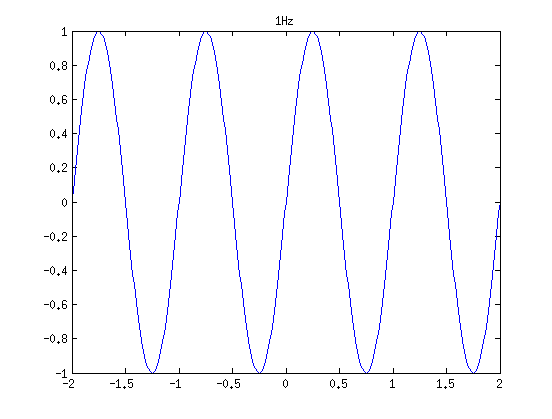
\includegraphics[width=0.48\textwidth]{sine1.png}%
}
\subfigure[]{%
  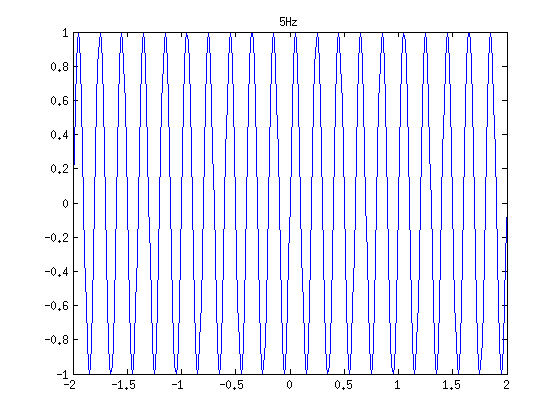
\includegraphics[width=0.48\textwidth]{sine2.png}%
}
%\caption{}
\label{fig:sines}
\end{figure}


\end{frame}





\end{document}
